%----------------------------------------------------------------------------------------
%	PACKAGES & THEMES
%----------------------------------------------------------------------------------------

\pdfminorversion=4
\documentclass[8pt]{beamer}

\usepackage{etex}
\mode<presentation> {

\usetheme{Vilanova}

}



\usepackage[french]{babel}
\usepackage[utf8]{inputenc}
\usepackage{array}
\usepackage{chronology}
\let\CHRONOLOGY\chronology
\let\endCHRONOLOGY\endchronology
\def\chronology{\shorthandoff{;}\CHRONOLOGY}
\def\endchronology{\endCHRONOLOGY\shorthandon{;}}
\usepackage{pstricks}
\usepackage{graphicx}
\usepackage{booktabs}
\usepackage{amsmath,amssymb,amsthm}
\usepackage{xcolor}
\usepackage{tikz}
\usetikzlibrary{arrows}
\usepackage{pifont}

\usepackage{listings,color}

\definecolor{listcomment}{rgb}{0.0,0.5,0.0}
\definecolor{listkeyword}{rgb}{0.0,0.0,0.5}
\definecolor{listnumbers}{gray}{0.65}
\definecolor{listlightgray}{gray}{0.955}
\definecolor{listwhite}{gray}{1.0}


\AtBeginSection[]
{
\addtocounter{framenumber}{-1}
\begin{frame}
\frametitle{Sommaire}
\tableofcontents[currentsection]
\end{frame}}

\title{Quoi de neuf dans Orfeo Toolbox ?}
\subtitle{Un logiciel libre pour le traitement d'images de télédétection}
\author{}
\date{}

\pgfdeclareimage[height=96mm,width=130mm]{background}{../OTB-General/images/fondsClairSansLogo}
\pgfdeclareimage[height=0.2cm]{cc}{../OTB-General/images/CC-licence.png}
\setbeamertemplate{background}{\pgfuseimage{background}}
\pgfdeclareimage[height=0.6cm]{logoIncrust}{../OTB-General/images/logoIncrust}
\pgfdeclareimage[height=0.6cm]{logo_cnes}{../OTB-General/images/logo_cnes}
\logo{
\begin{tabular}{p{0.22\textwidth}p{0.58\textwidth}p{0.1\textwidth}p{0.1\textwidth}}
\href{http://www.cnes.fr}{\pgfuseimage{logo_cnes}}
& \vspace{-0.03\textwidth} \scriptsize{} % date and event here
& \href{http://creativecommons.org/licenses/by-sa/3.0/}{\pgfuseimage{cc}} & \href{http://www.orfeo-toolbox.org}{\pgfuseimage{logoIncrust}}\\
\end{tabular}
}

\titlegraphic{\vspace*{-7em}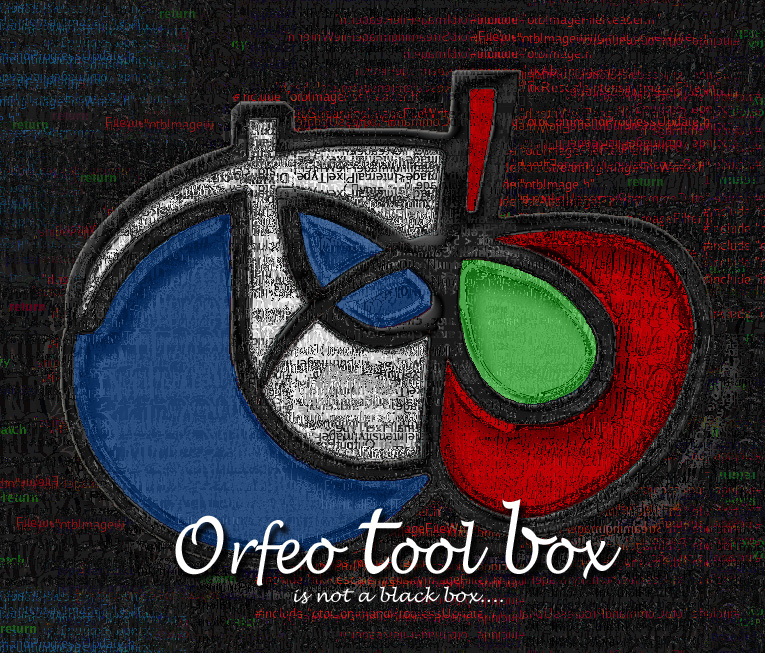
\includegraphics[width=.5\textwidth]{../OTB-General/images/LOGOTB_blackbox.png}}

\begin{document}
\begin{frame}
\titlepage
\end{frame}

\section*{Introduction}

\begin{frame}
\frametitle{Si vous ne retenez qu'une planche\ldots}
\begin{block}{L'Orfeo ToolBox est:}
\begin{itemize}
\item Une \textbf{bibliothèque de traitement d'images} pour la télédétection
\item \textbf{Un logiciel libre} diffusé sous licence CeCILL-v2 (équivalent à la GPL)
\item \textbf{Financée et développée par le CNES} (principalement)
\item Écrite en \textbf{C++} sur la base d'\href{www.itk.org}{ITK} (imagerie médicale)
\item Construite sur les épaules de géants (ITK, GDAL, OSSIM, OpenCV\ldots)
\item Conçue pour traiter de \textbf{gros volumes de données} de manière transparente grâce au traitement par morceaux et à la parallélisation
\end{itemize}
\end{block}

\begin{center}
{\huge\textcolor{red}{\href{http://www.orfeo-toolbox.org}{orfeo-toolbox.org}}}
\end{center}

\end{frame}

\begin{frame}
\frametitle{Pourquoi un logiciel libre ?}

\begin{block}{Diffusion maximale}
L'OTB est un logiciel à destination de tous les utilisateurs d'imagerie
spatiale. Sa diffusion large contribue au rayonnement des missions (Pléiades, Sentinels\ldots)
\end{block}

\begin{block}{Qualité et efficacité}
Le domaine fonctionnel de l'OTB est vaste, son développement nécessite du temps et de l'expertise. L'ouverture des sources:
\begin{itemize}
\item Favorise l'appropriation et la validation par la communauté des utilisateurs,
\item Favorise les contributions et les corrections de bugs par les utilisateurs,
\item Favorise la dissémination sur de multiples plate-formes.
\item ``The Cathedral \& the
  Bazaar''\footnote{\url{http://www.catb.org/esr/writings/cathedral-bazaar/}}:
  ``Publiez tôt, publiez souvent ``, ``s'appuyer sur la dynamique du projet''

\end{itemize}
\end{block}

\begin{block}{Démarche scientifique}
Comme l'OTB capitalise une partie de la R\&D du CNES en extraction d'information, l'ouverture des sources permet une démarche de \textbf{recherche reproductible}.
\end{block}

\end{frame}

\section{Fonctionnalités et utilisation}

\begin{frame}
\frametitle{Les grandes familles de fonctionnalités dans l'OTB (forcément incomplètes)}
\begin{itemize}
  \item Pré-traitements
  \item Manipulation d'images et de vecteurs
  \item Détection d'éléments saillants et calcul de primitives
  \item Détection de changement
  \item Réduction de la dimension, traitement hyperspectraux
  \item Segmentation
  \item Classification
\end{itemize}
$\Rightarrow$ Proche de l'état de l'art.
\end{frame}

\begin{frame}[plain]
\hspace*{-11mm}
    \includegraphics[keepaspectratio,height=1.1\paperheight]{../OTB-General/images/mayotte2012.png}
\end{frame}

\vspace*{-6.5mm}
\begin{frame}[plain]
\hspace*{-11mm}
    \includegraphics[keepaspectratio,height=1.1\paperheight]{../OTB-General/images/mayotte2013.png}
\end{frame}

\vspace*{-6.5mm}
\begin{frame}[plain]
\hspace*{-11mm}
    \includegraphics[keepaspectratio,height=1.1\paperheight]{../OTB-General/images/mayotte_mad.png}
\end{frame}

\vspace*{-6.5mm}
\begin{frame}[plain]
\hspace*{-11mm}
\includegraphics[keepaspectratio,height=1.1\paperheight]{../OTB-General/images/saint_paul_lsd.png}
\end{frame}

\vspace*{-6.5mm}
\begin{frame}[plain]
\hspace*{-11mm}
    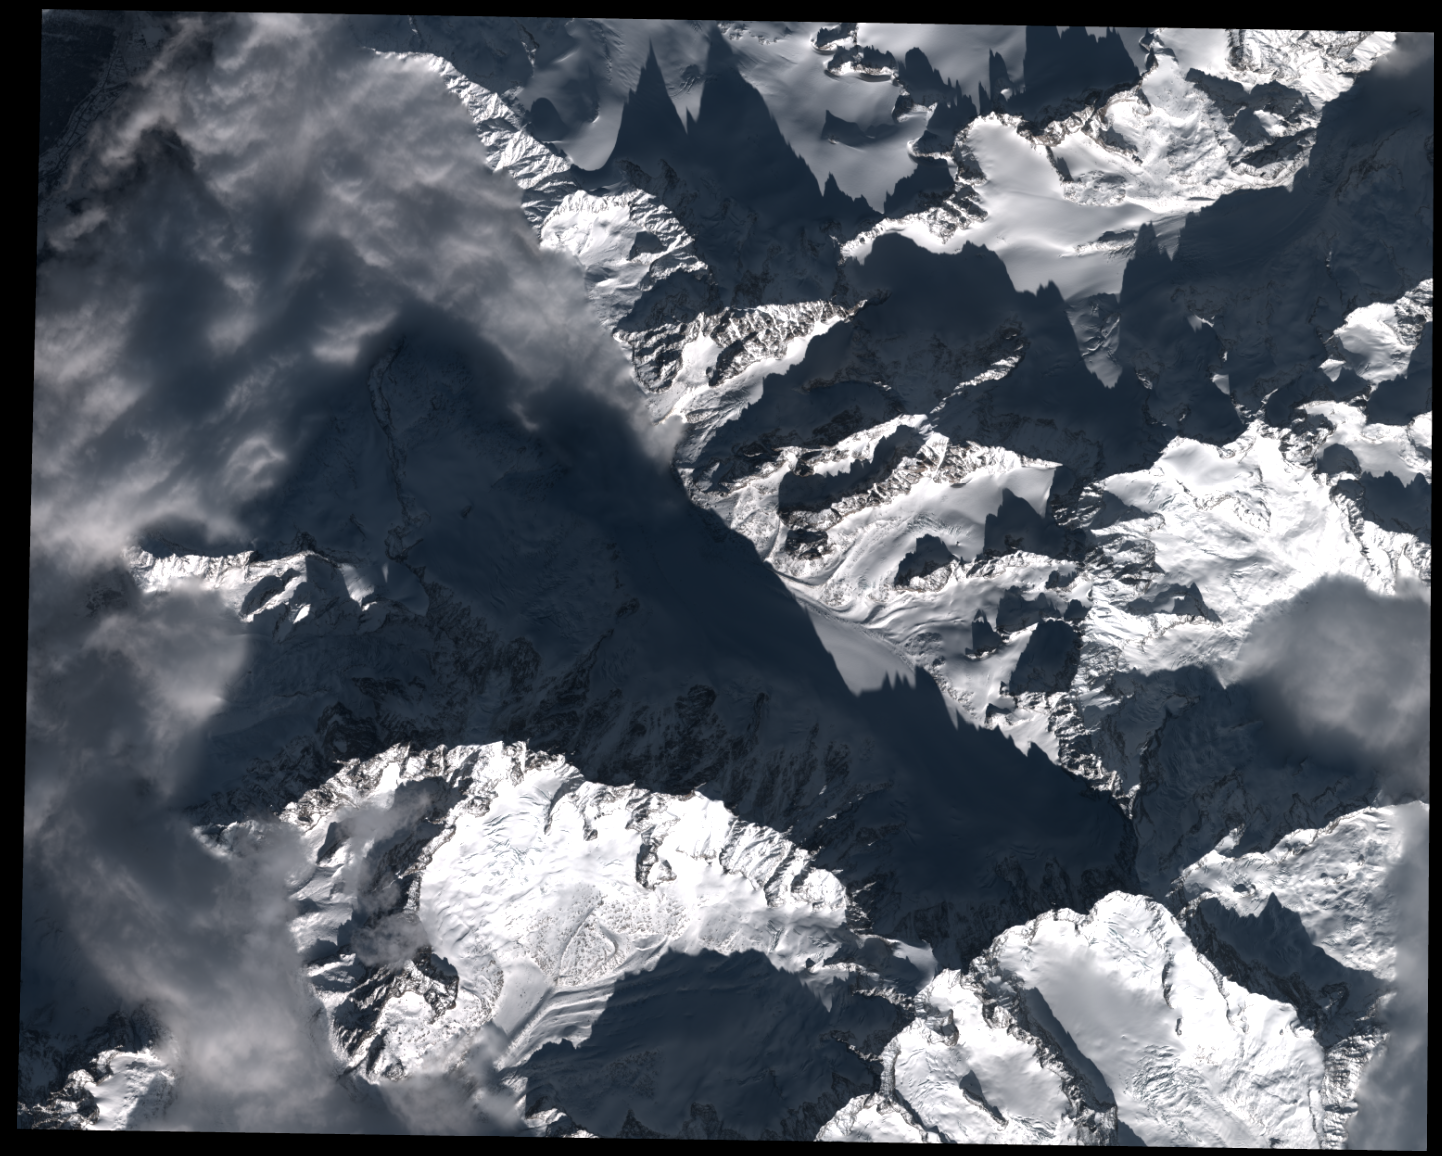
\includegraphics[keepaspectratio,width=1.005\paperwidth,height=1.1\paperheight]{../OTB-General/images/argentiere_left.png}
\end{frame}

\vspace*{-6.5mm}
\begin{frame}[plain]
\hspace*{-11mm}
    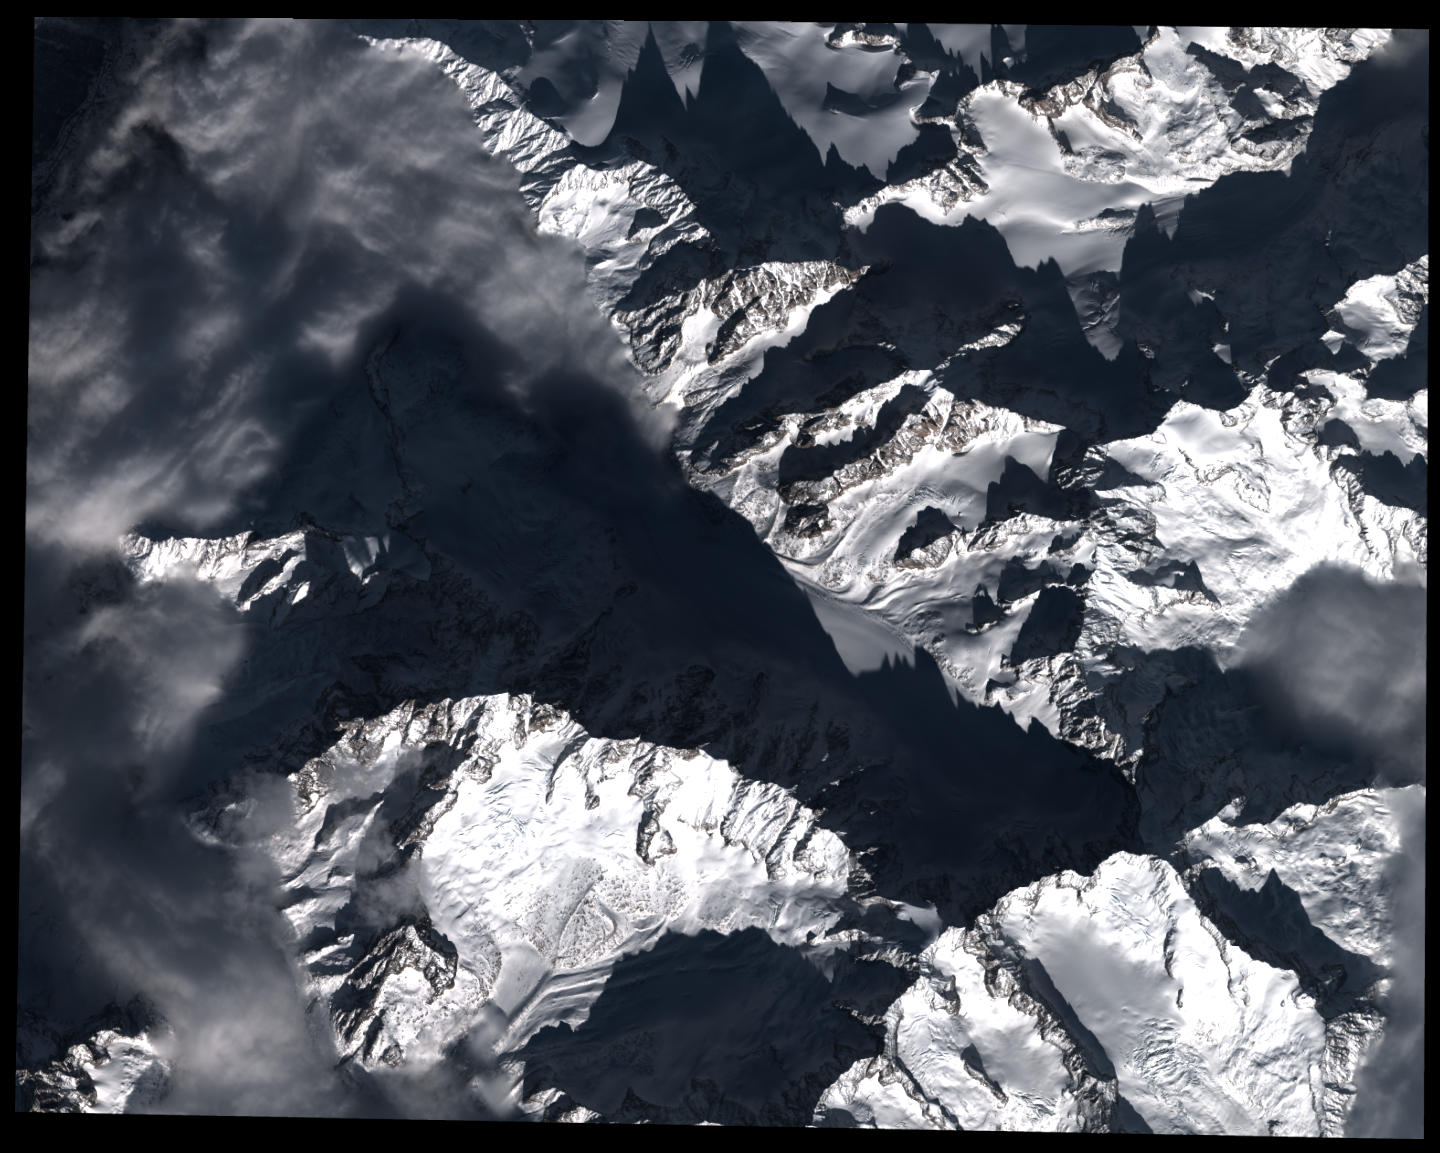
\includegraphics[keepaspectratio,width=1.005\paperwidth,height=1.1\paperheight]{../OTB-General/images/argentiere_right.png}
\end{frame}

\vspace*{-6.5mm}
\begin{frame}[plain]
\hspace*{-11mm}
    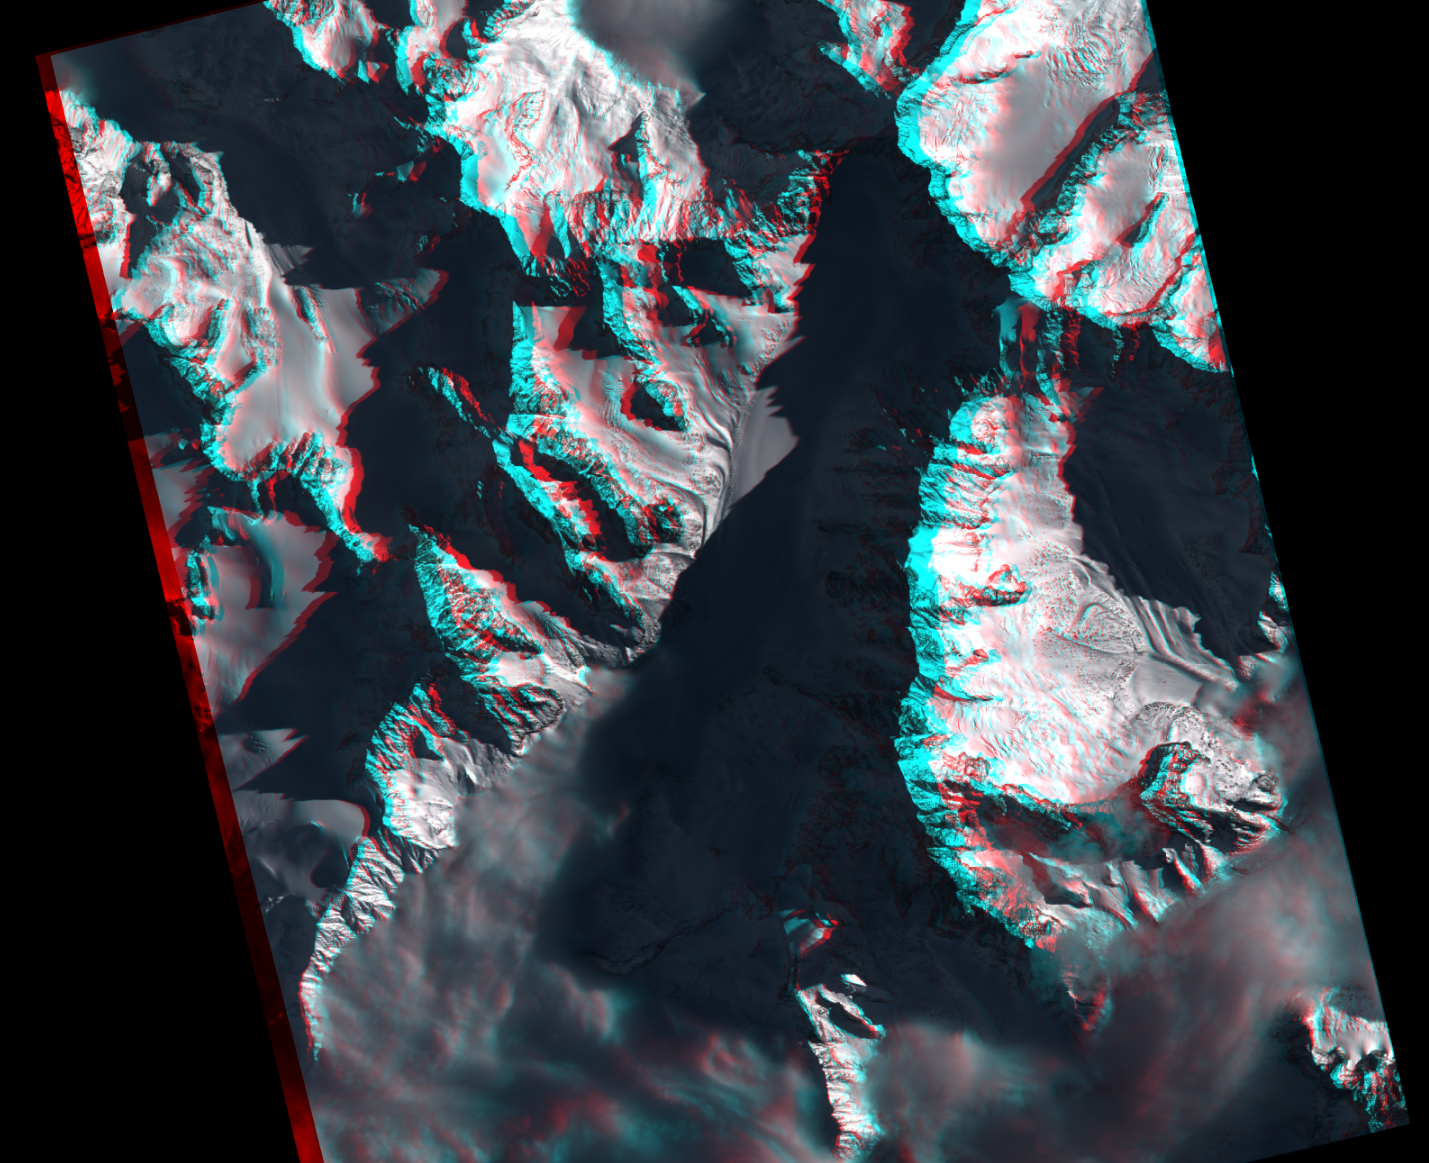
\includegraphics[keepaspectratio,width=1.005\paperwidth,height=1.1\paperheight]{../OTB-General/images/argentiere_anaglyphe.png}
\end{frame}

\begin{frame}
\frametitle{Comment utiliser l'Orfeo Toolbox?}
\vspace{-0.5cm}
\begin{center}
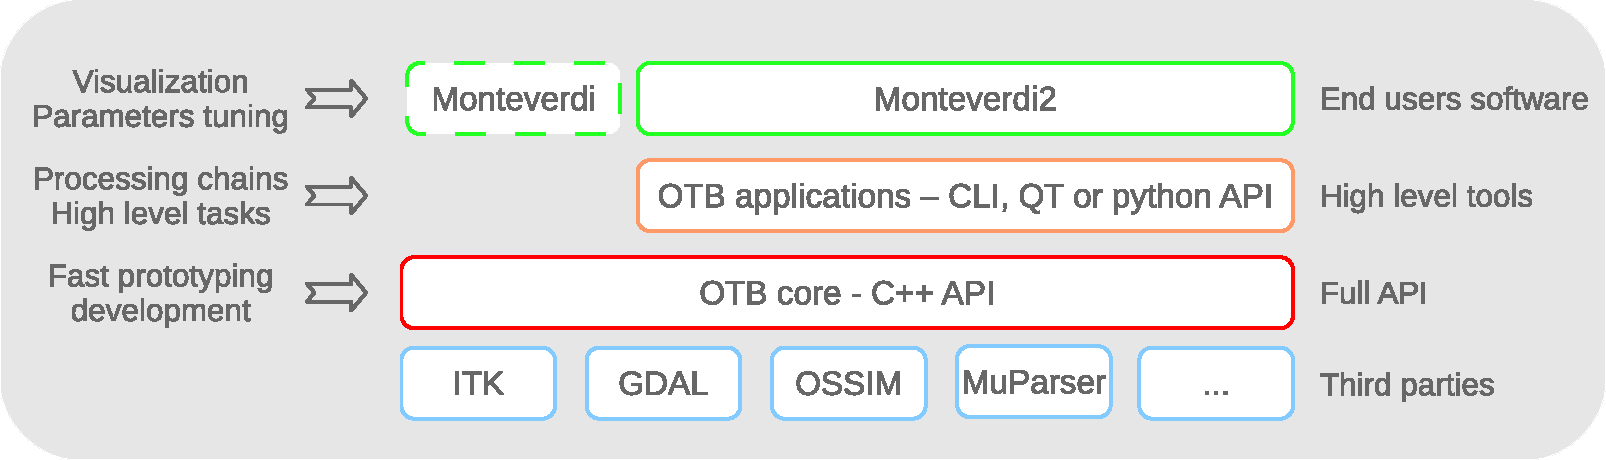
\includegraphics[width=\textwidth]{../OTB-General/images/sandwich.pdf}
\end{center}
\vspace{-0.5cm}
\begin{block}{Écrire son propre code}
 Flexible, à partir de la bibliothèque OTB, demande une connaissance en C++
\end{block}
\begin{block}{Utiliser les applications OTB}
 Fonctions de haut niveau (par ex. segmentation), appelable en ligne de commande, via une interface graphique, ou depuis Python. Peut être étendue (création d'applications)
\end{block}
\begin{block}{Utiliser le module Monteverdi (IHM)}
Visualisation, gestion persistante des données, \textcolor{red}{Accès à l'ensemble des applications}
\end{block}
\end{frame}

\begin{frame}[fragile]
\frametitle{Show me the code!}
\begin{lstlisting}[language=c++,breaklines=true,breakatwhitespace=true,frame = tb,framerule = 0.25pt,fontadjust,backgroundcolor={\color{listlightgray}},basicstyle = {\ttfamily\tiny},keywordstyle = {\ttfamily\color{listkeyword}\textbf},identifierstyle = {\ttfamily},commentstyle = {\ttfamily\color{listcomment}\textit},stringstyle = {\ttfamily},showstringspaces = false,showtabs = false,numbers = none,numbersep = 2pt, numberstyle={\ttfamily\color{listnumbers}},tabsize = 2]
#include "otbImage.h"
#include "otbImageFileReader.h"
#include "otbImageFileWriter.h"
#include "itkCannyEdgeDetectionImageFilter.h"
#include "itkRescaleIntensityImageFilter.h"

int main(int argc, char * argv[])
{
  typedef double                      PixelType;
  typedef otb::Image<PixelType>       ImageType;

  typedef unsigned char               OutputPixelType;
  typedef otb::Image<OutputPixelType> OutputImageType;

  typedef otb::ImageFileReader<ImageType> ReaderType;
  ReaderType::Pointer reader = ReaderType::New();

  reader->SetFileName(argv[1]);

  typedef itk::CannyEdgeDetectionImageFilter
  <ImageType, ImageType> FilterType;
  FilterType::Pointer filter = FilterType::New();

  filter->SetInput(reader->GetOutput());

  typedef otb::ImageFileWriter<OutputImageType> WriterType;
  WriterType::Pointer writer = WriterType::New();

  writer->SetFileName(argv[2]);

  writer->SetInput(filter->GetOutput());

  writer->Update();
}
\end{lstlisting}
\end{frame}

\begin{frame}
\frametitle{Les applications OTB: codées une fois, utilisables partout}
\begin{columns}
\column{0.5\textwidth}
\begin{itemize}
\item 87 applications sont livrées avec l'OTB
\item 1 application $=$ 1 librairie dynamique (plugin)
\item Les applications sont auto-descriptives et auto-documentées
\item Les applications peuvent etre étendues en dehors de l'OTB
\item Plusieurs interfaces sont disponibles pour utiliser les plugins:
\begin{itemize}
  \item Ligne de commande
  \item Interface Qt auto-générée
  \item Python
\end{itemize}
\item Les applications sont conçues pour une intégration facilitée dans des systèmes externes
\end{itemize}
\column{0.5\textwidth}
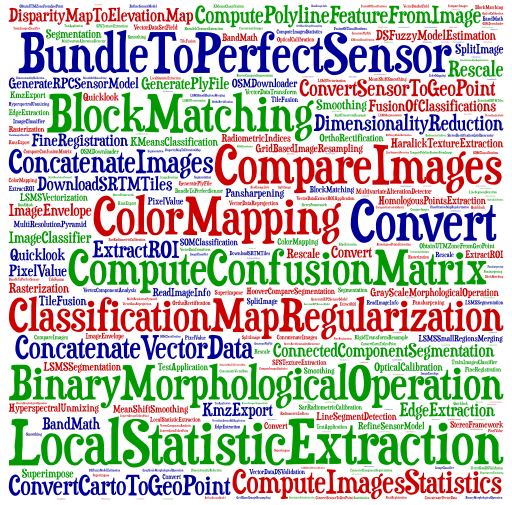
\includegraphics[width=\textwidth]{../OTB-General/images/cloud_applications.png}
\end{columns}
\end{frame}



\begin{frame}[fragile]
\frametitle{Applications OTB: Ligne de commande}
\begin{scriptsize}
\vspace{-0.5cm}\begin{verbatim}
$ otbcli_OrthoRectification

ERROR: Waiting for at least one parameter...
This is the OrthoRectification application, version 5.2.1
This application allows to ortho-rectify optical images from supported sensors.

Complete documentation: http://www.orfeo-toolbox.org/Applications/OrthoRectification.html

Parameters:
        -progress                <boolean>        Report progress
MISSING -io.in                   <string>         Input Image  (mandatory)
MISSING -io.out                  <string> [pixel] Output Image  [pixel=uint8/uint16/int16/uint32/int32/float/double] (default value is float) (mandatory)
        -map                     <string>         Output Cartographic Map Projection [utm/lambert2/lambert93/wgs/epsg] (mandatory, default value is utm)
        -map.utm.zone            <int32>          Zone number  (mandatory, default value is 31)
        -map.utm.northhem        <boolean>        Northern Hemisphere  (optional, off by default)
        -map.epsg.code           <int32>          EPSG Code  (mandatory, default value is 4326)
        -outputs.mode            <string>         Parameters estimation modes [auto/autosize/autospacing/outputroi/orthofit] (mandatory, default value is auto)
MISSING -outputs.ulx             <float>          Upper Left X  (mandatory)
MISSING -outputs.uly             <float>          Upper Left Y  (mandatory)
MISSING -outputs.sizex           <int32>          Size X  (mandatory)
MISSING -outputs.sizey           <int32>          Size Y  (mandatory)
MISSING -outputs.spacingx        <float>          Pixel Size X  (mandatory)
MISSING -outputs.spacingy        <float>          Pixel Size Y  (mandatory)
        -outputs.lrx             <float>          Lower right X  (optional, off by default)
        -outputs.lry             <float>          Lower right Y  (optional, off by default)
        -outputs.ortho           <string>         Model ortho-image  (optional, off by default)
        -outputs.isotropic       <boolean>        Force isotropic spacing by default  (optional, on by default)
        -outputs.default         <float>          Default pixel value  (optional, on by default, default value is 0)
        -elev.dem                <string>         DEM directory  (optional, off by default)
        -elev.geoid              <string>         Geoid File  (optional, off by default)
        -elev.default            <float>          Default elevation  (mandatory, default value is 0)
        -interpolator            <string>         Interpolation [bco/nn/linear] (mandatory, default value is bco)
\end{verbatim}
\end{scriptsize}
\end{frame}

\begin{frame}[fragile]
\frametitle{Applications OTB: Interface graphique}
\begin{center}
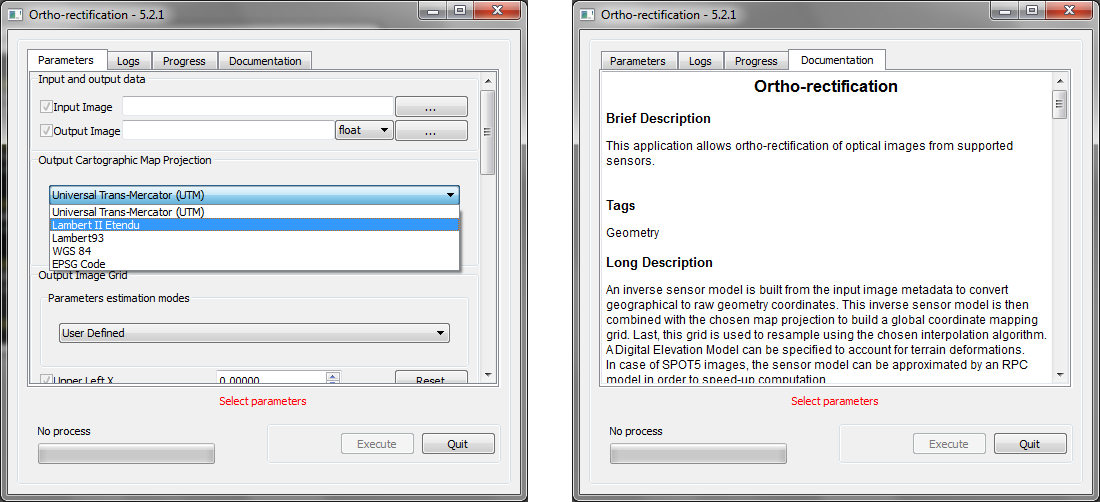
\includegraphics[width=1\textwidth]{../OTB-General/images/otbgui.png}
\end{center}
\end{frame}

\begin{frame}[fragile]
\frametitle{Applications OTB: Interface Python}
\begin{lstlisting}[language=python,breaklines=true,breakatwhitespace=true,frame = tb,framerule = 0.25pt,fontadjust,backgroundcolor={\color{listlightgray}},basicstyle = {\ttfamily\tiny},keywordstyle = {\ttfamily\color{listkeyword}\textbf},identifierstyle = {\ttfamily},commentstyle = {\ttfamily\color{listcomment}\textit},stringstyle = {\ttfamily},showstringspaces = false,showtabs = false,numbers = none,numbersep = 6pt, numberstyle={\ttfamily\color{listnumbers}},tabsize = 2]
#!/usr/bin/python

# Import the otb applications package
import otbApplication

# The following line creates an instance of the OrthoRectification application
OrthoRectification = otb.Registry.CreateApplication("OrthoRectification")

# The following lines set all the application parameters:
OrthoRectification.IO.IN = "QB_TOULOUSE_MUL_Extract_500_500.tif"
OrthoRectification.IO.OUT = "QB_Toulouse_ortho.tif"

app.MAP = 'epsg'
app.MAP.EPSG.CODE = 32768

# The following line execute the application
OrthoRectification.ExecuteAndWriteOutput()
\end{lstlisting}
\end{frame}

%\vspace*{-6.0mm}
\begin{frame}
\frametitle{Monteverdi (accès aux applications OTB)}
\begin{minipage}[t][6cm][t]{\textwidth}
\begin{center}
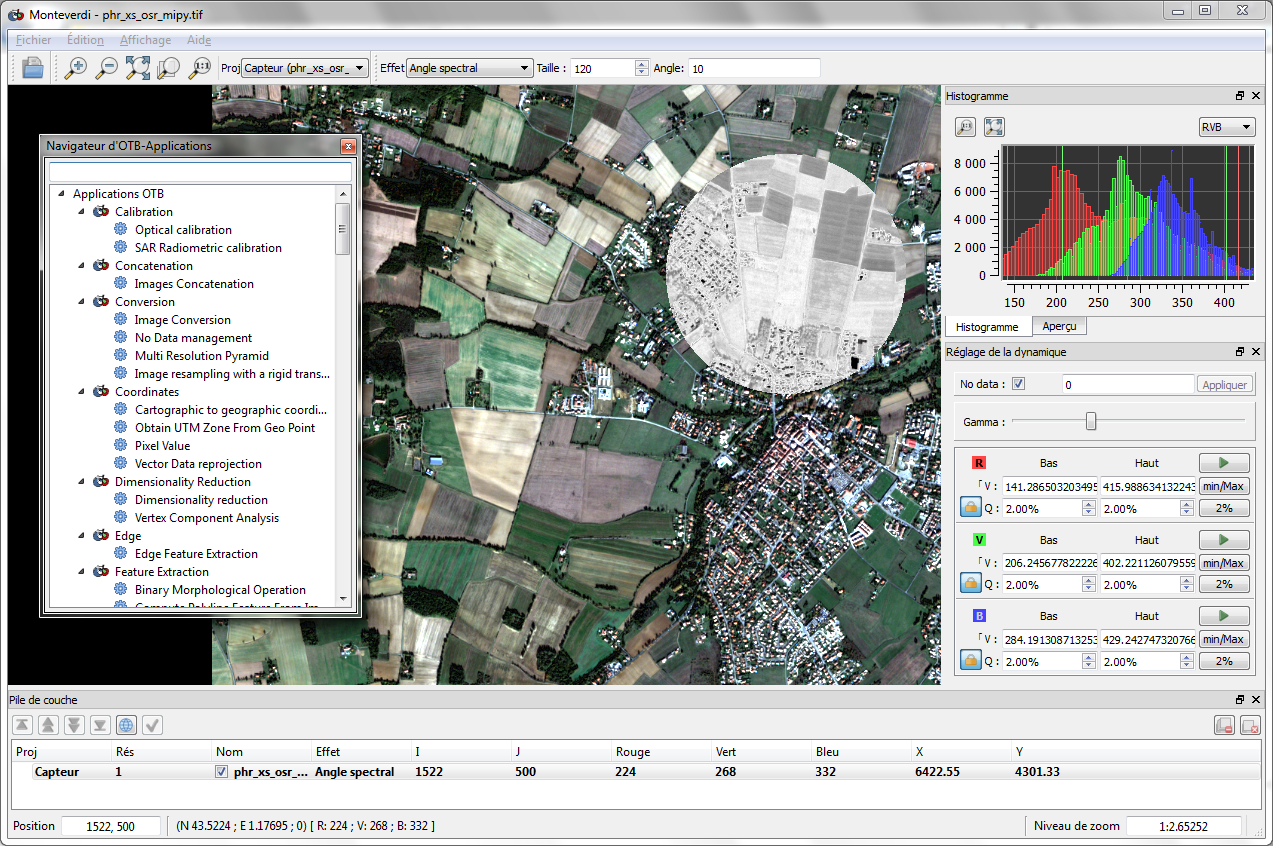
\includegraphics[width=1.0\textwidth]{../OTB-General/images/monteverdi.png}
\end{center}
\end{minipage}
\end{frame}

%\vspace*{-3.0mm}
\begin{frame}
  \frametitle{QGIS (accès aux applications OTB)}
\begin{minipage}[t][6cm][t]{\textwidth}
\begin{center}
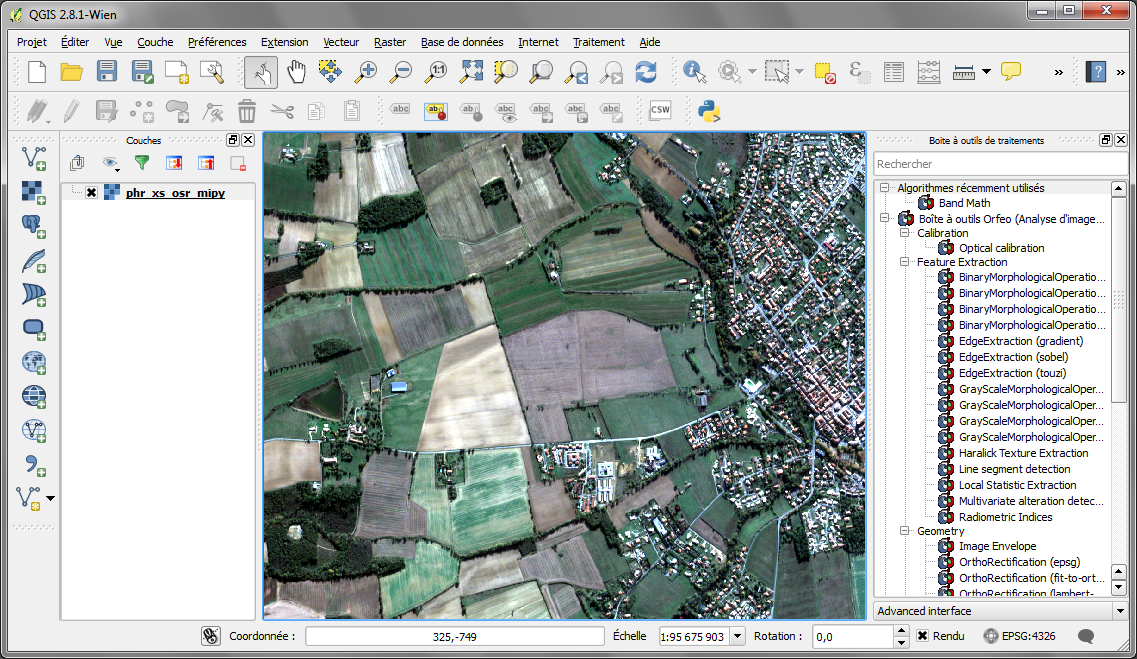
\includegraphics[width=1\textwidth]{../OTB-General/images/otb_in_qgis.png}
\end{center}
\end{minipage}
\end{frame}

\section{Quoi de neuf depuis 5.0 ?}

\begin{frame}
\frametitle{5.0 (Mai 2015)}
\begin{block}{Modularité}
\begin{itemize}
\item Une meilleure organisation du code, en modules cohérents (124 modules et
    16 groupes) contenants sources, tests et applications.
\item Gestion des dépendances
\item Contributions externes: \url{https://www.orfeo-toolbox.org/external-projects/}
\end{itemize}
\end{block}

\begin{block}{SuperBuild}
\begin{itemize}
\item Il n'y a plus de logiciels tiers dans l'OTB
\item Il existe un projet séparé appelé Superbuild, qui télécharge, configure, compile et installe chaque dépendance dans sa bonne version
\item On peut ainsi compiler une OTB complète avec très peu de pré-requis (cmake, gcc, zlib, curl), et totalement automatiquement
\item Il existe également un mode \textit{offline} pour compiler l'OTB sans
  accès internet (en avion par exemple).
\end{itemize}
\end{block}
\end{frame}

\begin{frame}
\frametitle{5.2 (Décembre 2015)}
\begin{block}{OTB}
\begin{itemize}
\item Nouvelles applications pour le traitement SAR (polarimétrie)
\item Support des produits Sentinel-1
\item Calibration radiométrique image SAR (Sentinel1 et Radarsat2)
\item Méthodes pour le filtrage du Speckle (Frost, Lee, GammaMAP, Kuan)
\item Mode régression et carte de confiance pour la classification
\item Amélioration accès OTB en Python
\item Compatibilité avec GDAL 2.0 et support des images Sentinel-2
\end{itemize}
\end{block}

\begin{block}{Monteverdi 3.0}
\begin{itemize}
\item Léger et performant
\item Affichage mosaïque d'images ou série multi-temporelle
\item Outils de visualisation performants (contraste local, gradient\ldots)
\item Accès aux applications OTB
\end{itemize}
\end{block}
\end{frame}

\begin{frame}
\frametitle{5.4 (Mai 2016)}
\begin{block}{OTB}
\begin{itemize}
\item Passage à un cycle de release fixe (3 mois)
\item Intégration du composant de visualisation
\item Nouveau framework d'échantillonage
\item Compilation externe des modules externes
\item Green dashboard
\item Nouvelles décompositions SAR: Barnes, Huynen, Pauli
\end{itemize}
\end{block}

\begin{block}{Monteverdi 3.2}
\begin{itemize}
\item Capture d'écran
\item Génération d'overviews
\item Import fichiers CDS
\item Ajout au SuperBuild
\end{itemize}
\end{block}
\end{frame}

\begin{frame}
\frametitle{Communauté OTB}
\begin{center}
Documentation, blog, wiki, git, bugtracker, dashboard, listes de diffusion:
{\huge\textcolor{red}{\href{http://www.orfeo-toolbox.org}{orfeo-toolbox.org}}}
\end{center}

\begin{block}{Évènements}
\begin{description}
  \item[Journées Utilisateurs OTB] {Du 7 au 9 Juin 2016 à Toulouse}
  \item[École d’été OTB et MicMac] {Du 4 au 8 Juillet 2016 à l'ENSG Paris}
\end{description}
\end{block}
\end{frame}

\end{document}
